\documentclass[12pt,english,a4paper]{book}
\usepackage[T1]{fontenc}
\usepackage[latin9]{inputenc}
\usepackage{graphicx}
\usepackage{amsfonts}
\usepackage{textcomp}
\usepackage{color}
\usepackage{calc}
\usepackage{longtable}
\usepackage{hyperref}
\usepackage{graphics}
\DeclareGraphicsExtensions{.jpg}
\DeclareGraphicsExtensions{.png}
\hypersetup{colorlinks=true, linkcolor=blue, filecolor=blue, pagecolor=blue, urlcolor=blue}

%%%%\%%%%%%%% titre, auteurs, date, etc...%%%%%%%%%%%%%%%%%%
\title{\Huge The CanFestival CANOpen stack manual}
\author{Edouard TISSERANT}
\date{\today}

\setcounter{secnumdepth}{5}
\renewcommand\thesection{\arabic{section} -}
\renewcommand\thesubsection{\arabic{section}.\arabic{subsection})}
\renewcommand\thesubsubsection{\arabic{section}.\arabic{subsection}.\arabic{subsubsection})}
\renewcommand\theparagraph{\alph{paragraph})}
\renewcommand\thesubparagraph{\roman{subparagraph})}

\newcommand{\canopen}{CANopen }

\begin{document}
{\centering\textsf{\huge The CanFestival \canopen stack manual.}}

\renewcommand{\contentsname}{CanFestival v3.0 Manual}
\setcounter{tocdepth}{2} \tableofcontents{}

\clearpage{}

\section{Introduction}

CanFestival is an OpenSource (LGPL and GPL) \canopen framework.

\subsection{The CanFestival project}

This project, initiated by Edouard TISSERANT in 2001, has grown thanks
to Francis DUPIN and other contributors.

Today, CanFestival focuses on providing an ANSI-C platform independent
\canopen stack that can be implemented as master or slave nodes on
PCs, Real-time IPCs, and Microcontrollers.


\subsection{What is \canopen}

CANopen is a CAN based high level protocol. It defines some protocols
to :

\begin{enumerate}
\item Configure a CAN network. 
\item Transmit data to a specific node or in broadcast. 
\item Administrate the network. For example detecting a not responding node. 
\end{enumerate}
The documentation can be found on the CAN in Automation website :

\href{http://www.can-cia.de/canopen}{http://www.can-cia.de/canopen}

The most important document about \canopen is the normative CiA Draft
Standard 301, version 4.02. You can now download the specification
from the CAN in Automation website at no cost.

To continue reading this document, let us assume that you have read
some papers introducing \canopen .


\section{CanFestival Features}


\subsection{Tools }

The \canopen library is coming with some tools :

\begin{enumerate}
\item Object Dictionary editor GUI. WxPython Model-View-Controler based
GUI, that helps a lot in generating object dictionary source code for
each node. 
\item A configure script, that let you chose compile time options such as
target CPU/HOST, CAN and TIMER drivers.\\
 This script has not been generated with autoconf, it has been made
keeping micro-controller target in mind. 
\end{enumerate}

\subsection{Multi-Platform}

\begin{enumerate}
\item Library source code is C-ANSI. 
\item Driver and examples coding conventions merely depend on target specific
contributor/compiler. 
\item Unix compatible interfaces and examples should compile and run on
any Unix system (tested on GNU/Linux and GNU/FreeBSD). 
\end{enumerate}

\subsection{\canopen standard conformance}

\subsubsection{DS-301}

Supported features should conform to DS301. V.4.02 13 february 2002. 

\begin{enumerate}
\item NMT master and slave
\item Heartbeat consumer and producer
\item NodeGuard slave reponder and basic master without tracking
\item SYNC service
\item SDO multiples client and server, segmented and expedited
\item PDO : TPDO and RPDO, with respect to transmission type
\item PDO mapping from/to OD variables bit per bit. 
\item EMCY : Send and receive and keeps track of emergency objects
\item Data types : 8 to 64 bits values, fixed length strings.
\end{enumerate}

\subsubsection{DS-302}

Only concise DFC is supported.

\subsubsection{DS-305}

LSS services are fully supported although they have to be enabled at compile time. Additionally, FastScan LSS service is also optionally enabled. 

\section{How to start}

\subsection{Host requirements}

What you need on your development workstation.

\subsubsection{Object Dictionary Editor GUI}

\begin{enumerate}
\item Python, with 
\item wxPython modules installed (at least version 2.6.3).
\item Gnosis xml tools. (Optional can also be installed locally to the project
automatically with the help of a Makefile. Please see {}``Using Dictionary
Editor GUI'' ) 
\end{enumerate}

\subsubsection{Linux and Unix-likes}

\begin{enumerate}
\item Linux, FreeBSD, Cygwin or any Unix environment with GNU toolchain. 
\item The GNU C compiler (gcc) or any other ANSI-C compiler for your target
platform. 
\item Xpdf, and the official 301\_v04000201.pdf file in order to get GUI
context sensitive help. 
\item GNU Make 
\item Bash and sed 
\end{enumerate}

\subsubsection{Windows (for native win32 target)}

\begin{enumerate}
\item Visual Studio Express 2005 or worst.
\item Microsoft platform SDK (requires Genuine Advantage)
\item Cygwin (for configuration only)
\item MinGW/MSYS
\end{enumerate}

\section{Understanding Canfestival}

\subsection{CanFestival Project tree layout}
Simplified directory structure.
\begin{verbatim}
./src ANSI-C source of \canopen stack
./include Exportables Header files
./drivers Interfaces to specific platforms/HW
./drivers/unix Linux and Cygwin OS interface
./drivers/win32 Native Win32 OS interface
./drivers/timers_xeno Xenomai timers/threads (Linux only)
./drivers/timers_rtai Rtai timers/threads (Linux only)
./drivers/timers_kernel Linux kernel timer/threads
./drivers/timers_unix Posix timers/threads (Linux, Cygwin)
./drivers/can_virtual_kernel Fake CAN network (kernel space)
./drivers/can_serial Serial point to point and PTY hub (*nix only)
./drivers/can_peak_linux PeakSystem CAN library interface
./drivers/can_peak_win32 PeakSystem PCAN-Light interface
./drivers/can_uvccm_win32 Acacetus's RS232 CAN-uVCCM interface
./drivers/can_virtual Fake CAN network (Linux, Cygwin)
./drivers/can_vcom VScom VSCAN interface
./drivers/hcs12 HCS12 full target interface
./examples Examples
./examples/TestMasterSlave 2 nodes, NMT SYNC SDO PDO, win32+unix
./examples/TestMasterSlaveLSS 3 nodes, NMT SYNC SDO PDO LSS, win32+unix
./examples/TestMasterMicroMod 1 node, control Peak I/O Module, unix
./examples/gene_SYNC_HCS12 Just send periodic SYNC on HCS12
./examples/win32test Ask some DS301 infos to a node (win32)
./objdictgen Object Dictionary editor GUI
./objdictgen/config Pre-defined OD profiles
./objdictgen/examples Some examples/test OD
./doc Documentation source
\end{verbatim}



\subsection{Implement CanFestival in your application}

\begin{center}
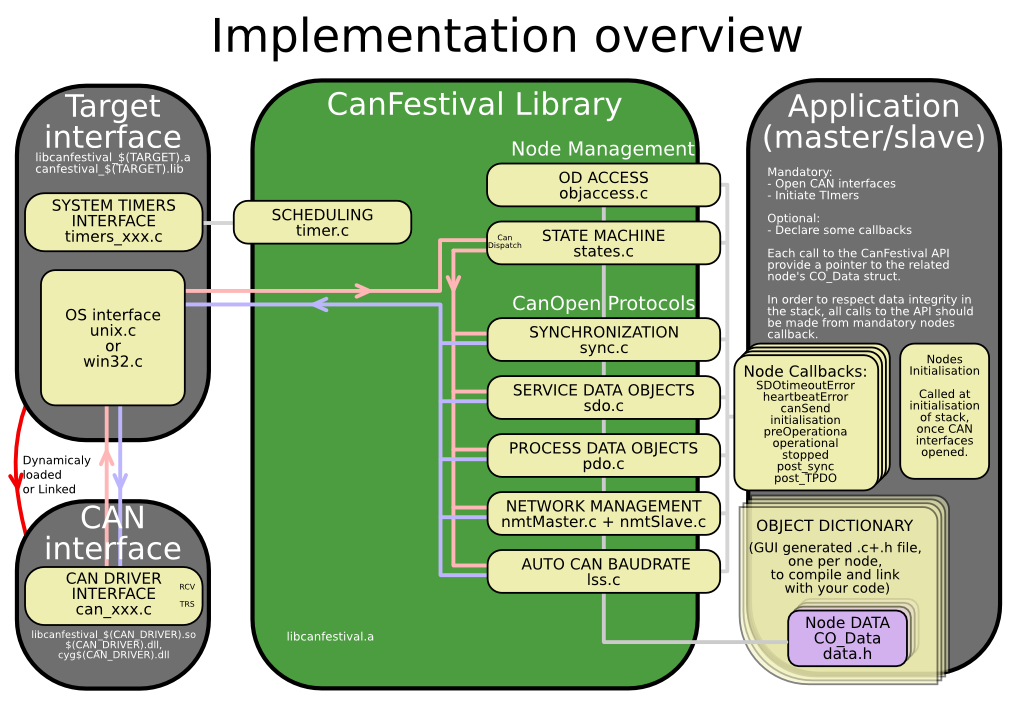
\includegraphics[width=12cm]{Pictures/10000201000003F9000002CF880931E7} 
\par\end{center}

\bigskip{}



\subsection{CanFestival CAN interfaces}

Because most CAN controllers and drivers implement FIFOs, CanFestival
consider sending message as a non blocking operation.

In order to prevent reentrant calls to the stack, messages reception
is implemented differently on {\textmu}C and OS.:

\begin{enumerate}
\item {\textmu}C must provide interruption masking, mutually excluding timer and CAN receive interrupts.\\



\begin{center}
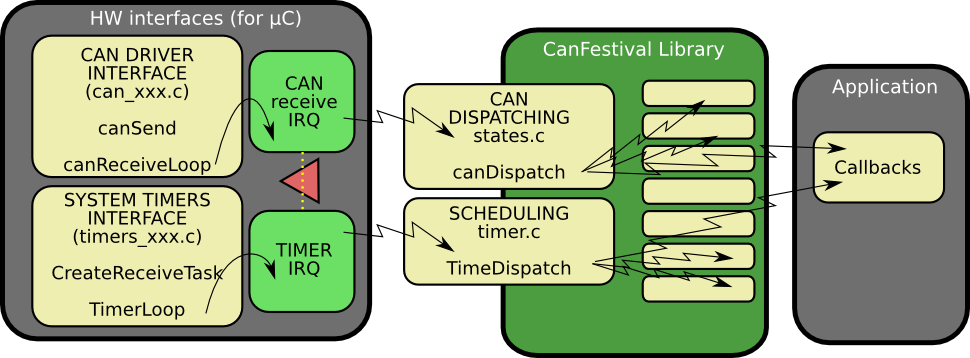
\includegraphics[width=12cm]{Pictures/10000201000003CA0000016604E6A5EF} 
\par\end{center}

\item OS must provide a receive thread, a timer thread and a mutex. CAN
reception should be a blocking operation.\\



\begin{center}
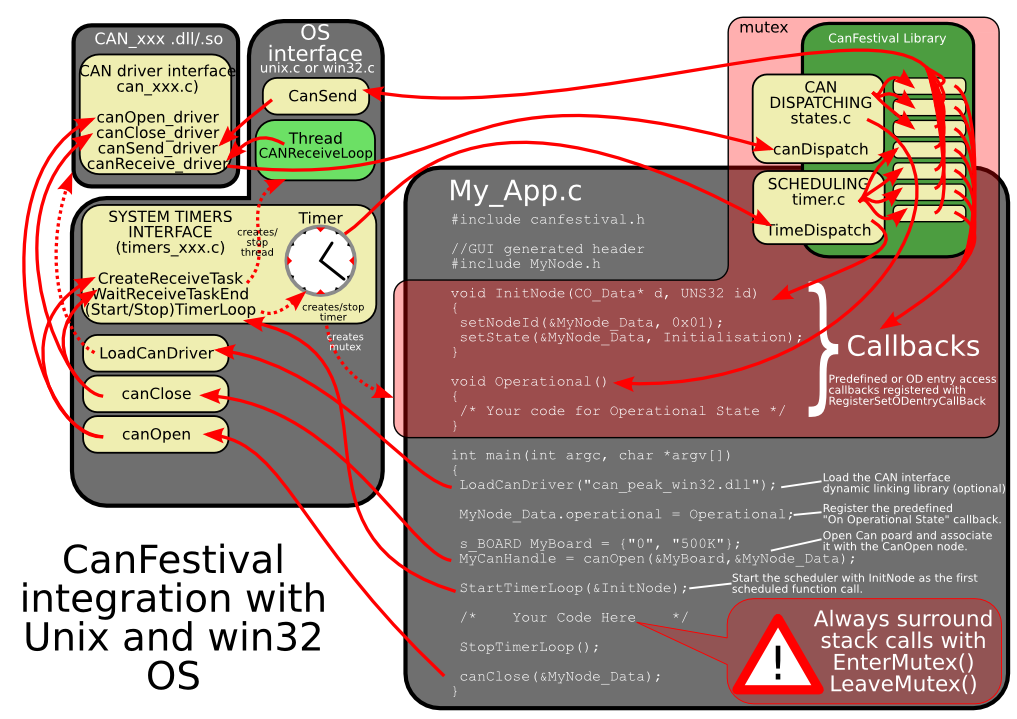
\includegraphics[width=12cm]{Pictures/10000201000003F9000002CF8B0CDAEA} 
\par\end{center}

\end{enumerate}

\subsection{CanFestival event scheduling}

A \canopen node must be able to take delayed actions.

For instance, periodic sync emission, heartbeat production or SDO timeout
need to set some alarms that will be called later and do the job.

{\textmu}C generally do not have enough free timers to handle all
the \canopen needs directly. Moreover, CanFestival internal data
may be corrupt by reentrant calls.

CanFestival implement a micro -scheduler (timer.c). It uses only one
timer to mimic many timers. It manage an alarm table, and call alarms
at desired time.

\begin{center}
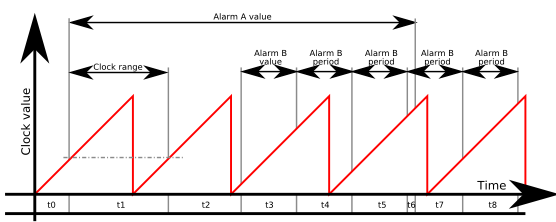
\includegraphics[width=12cm]{Pictures/100000000000022C000000DEDAD2140C} 
\par\end{center}

Scheduler can handle short clock value ranges limitation found on
some {\textmu}C. As an example, value range for a 16bit clock counter
with 4{\textmu}s tick is crossed within 0.26 seconds... Long alarms
must be segmented.

Chronogram illustrate a long alarm (A) and a short periodic alarm
(B), with a A value {\textgreater} clock range {\textgreater}
B value. Values t0...t8 are successive setTimer call parameter values.
t1 illustrates an intermediate call to TimeDispatch, caused by a delay
longer than clock range. Because of long alarm segmentation, at the
end of t1, TimeDispatch call will not trig any alarm callback.

\begin{center}
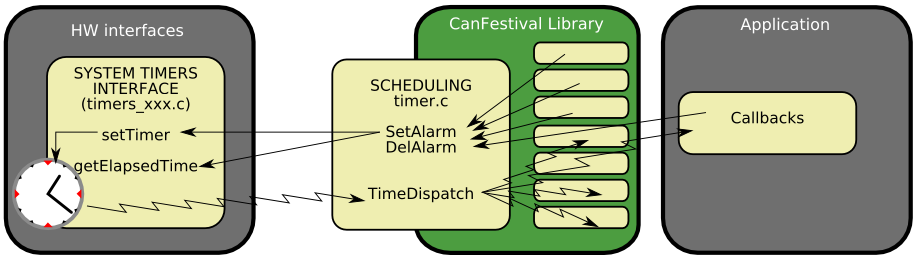
\includegraphics[width=12cm]{Pictures/1000000000000396000000FFC42573DA} 
\par\end{center}


\section{Linux Target}

Linux target is default configure target.


\subsection{Linux Compilation and installation}

Call ./configure -- help to see all available compile time options.

After invoking ./configure with your platform specific switches, just
type make.



\begin{verbatim}
	./configure [options]
	make
	make install
\end{verbatim}




\subsubsection{Standard Linux node}


\begin{verbatim}
	./configure --timers=unix
\end{verbatim}


To do a \canopen node running on PC -Linux, you need :

\begin{enumerate}
\item A working linux distribution 
\item One or more Peak system PC CAN interface and the last Peak Linux driver
installed. 
\end{enumerate}

\subsubsection{Real -Time Linux node}

With Xenomai :
\begin{verbatim}
	./configure --timers=xeno
\end{verbatim}
With Rtai :
\begin{verbatim}
	./configure --timers=rtai
\end{verbatim}

To do a \canopen node running on PC -Linux, you need :

\begin{enumerate}
\item A working Linux distribution patched with XENOMAI (2.1 or greater) or RTAI (3.6). 
\item One or more Peak system PC CAN interface and the last Peak Real Time
Linux driver installed. 
\end{enumerate}

\subsubsection{Linux kernel node}

To do a CANopen node running on PC-Linux in kernel space, you need:


\begin{enumerate}
\item A working Linux distribution with pre-built 2.6.x.x kernel sources
\item A CAN card driver compatible with CanFestival
\end{enumerate}


\subsubsection{CAN devices}
Currently supported CAN devices and corresponding configure switch:

\paragraph{Peak systems}
\begin{verbatim}
	./configure --can=peak_linux
\end{verbatim}
PeakSystems CAN interface is automatically chosen as default CAN interface
if libpcan is present in the system.

Please download driver at \href{http://www.peak-system.com/linux}{http://www.peak
-system.com/linux} and follow instructions in order to install driver
on your system.

\paragraph{Socket-Can (http://socketcan.berlios.de)}
\begin{verbatim}
	./configure --can=socket
\end{verbatim}

\paragraph{Serial}
\begin{verbatim}
	./configure --can=serial
\end{verbatim}
The CAN serial driver implements a 1:1 serial connection between 2 CAN devices.
For example, you can connect 2 CANFestival applications via a NULL modem cable.

Also with this driver comes a software hub, for up to 16 CANFestival apps to 
be connected on a single PC, with an optional connection to another CAN driver.
Note that only the serial driver is supported at this time.  The hub uses ptys 
(pseudo ttys) available on a *nix like system.

\paragraph{LinCan}
\begin{verbatim}
	./configure --can=lincan
\end{verbatim}

\paragraph{Virtual CAN interfaces (for test/debug)}
\begin{verbatim}
	./configure --can=virtual
		or, for kernel space:
	./configure --can=kernel_virtual
\end{verbatim}
Virtual CAN interface use Unix pipes to emulate a virtual CAN network.
Each message issued from a node is repeat to all other nodes. Currently
only works with nodes running in the same process, and does not support
work with Xenomai or RTAI.

\paragraph{VScom}
\begin{verbatim}
	./configure --can=vscom
\end{verbatim}
The VSCAN API archive will be automatically downloaded and decompressed (unzip required). See \href{http://www.vscom.de/1_1_05.htm}{www.vscom.de} for available adapters.

\subsubsection{LSS services}
Canfestival optionally supports LSS services but they must be enabled.
\begin{verbatim}
	./configure --enable-lss
\end{verbatim}

Additionally, the FastScan LSS service can also be enabled.
\begin{verbatim}
	./configure --enable-lss --enable-lss-fs
\end{verbatim}

\subsection{Testing your CanFestival installation}

\subsubsection{User space}

Sample provided in /example/TestMasterSlave is installed into your
system during installation.


\begin{verbatim}
	TestMasterSlave
\end{verbatim}


Default CAN driver library is libcanfestival\_can\_virtual.so., which
will simply pass CAN messages through Unix pipes between Master and
Slave.

You may also want to specify different can interface and define some
CAN ports. Another example using Peak{\textquotesingle}s dual PCMCIA
(configure and install with --can=peak) :


\begin{verbatim}
	TestMasterSlave -l libcanfestival_can_peak.so -s 40 -m 41
\end{verbatim}

If the LSS services are enabled the sample provided in /example/TestMasterSlaveLSS will be also installed. It behaves the same as TestMasterSlave except that there are 2 slave nodes without a valid nodeID so the the initializations is done via  the LSS services. If FastScan optional service is enabled the example will use it. 

\subsubsection{Kernel space}


\begin{verbatim}
	example/kerneltest
\end{verbatim}


It's based on TestMasterSlave example
and has the same functionality. Uses virtual can driver as default
too. After successful installation you can insert the module by typing:
modprobe canf\_ktest Module control is done by simple console 'canf\_ktest\_console'
which is used to start/stop sending data.


\section{Windows Targets}

CanFestival can be compiled and run on Windows platform. It is possible
to use both Cygwin and win32 native runtime environment.

\subsection{Object Dictionary Editor GUI installation.}

Please refer to \hyperlink{a821UsingDictionaryEditorGUIoutline}{8.2.1)Using
Dictionary Editor GUI}

\subsection{CYGWIN}

\subsubsection{Requirements}

Cygwin have to be installed with those packages :

\begin{enumerate}
\item gcc 
\item unzip 
\item wget 
\item make 
\end{enumerate}
Currently, the only supported CAN devices are PeakSystems ones, with
PcanLight driver and library.

Please download driver at \href{http://www.peak-system.com/themen/download_gb.html}{http://www.peak
-system.com/themen/download\_gb.html} \ and follow instructions
in order to install driver on your system.

Install Cygwin as required, and the driver for your Peak CAN device.

Open a Cygwin terminal, and follow those instructions:


\subsubsection{Cygwin configuration and compilation}


\paragraph{A single node with PcanLight and Peak CAN -USB adapter}

Download the PCAN-Light Zip file for your HW ( URL from download
page ):


\begin{verbatim}
	wget http://www.peak -system.com/files/usb.zip
\end{verbatim}


Extract its content into your cygwin home (it will create a {}``Disk''
directory):


\begin{verbatim}
	unzip usb.zip
\end{verbatim}


Configure CanFestival3 providing path to the desired PcanLight implementation:


\begin{verbatim}
	cd CanFestival -3
	export PCAN_INCLUDE=~/Disk/PCAN-Light/Api/
	export PCAN_HEADER=Pcan_usb.h
	export PCAN_LIB=~/Disk/PCAN-Light/Lib/Visual\ C++/Pcan_usb.lib
	./configure --can=peak_win32
	make
\end{verbatim}


In order to test, you have to use another CanFestival node, connect
with a CAN cable.


\begin{verbatim}
	cp ~/Disk/PCAN-Light/Pcan_usb.dll .
	./examples/TestMasterSlave/TestMasterSlave \
	-l drivers/can\_peak\_win32/cygcan\_peak\_win32.dll \
	-S 500K -M none
\end{verbatim}


Then, on the other node :


\begin{verbatim}
	./TestMasterSlave -l my_driver.so -S none -M 500K
\end{verbatim}


Now messages are being exchanged between master and slave node.

\paragraph{Two nodes with PcanLight and Peak dual PCMCIA -CAN adapter}

Download the PCAN-Light Zip file for your HW ( URL from download
page ):


\begin{verbatim}
	wget http://www.peak-system.com/files/pccard.zip
\end{verbatim}


Extract its content into your cygwin home (it will create a {}``Disk''
directory):


\begin{verbatim}
	unzip pccard.zip
\end{verbatim}


The configure CanFestival3 providing path to the desired PcanLight
implementation:


\begin{verbatim}
	export PCAN_INCLUDE=~/Disk/PCAN-Light/Api/
	export PCAN_HEADER=Pcan_pcc.h
	export PCAN_LIB=~/Disk/PCAN-Light/Lib/Visual\ C++/Pcan_pcc.lib
	export PCAN2_HEADER=Pcan_2pcc.h
	export PCAN2_LIB=~/Disk/PCAN-Light/Lib/Visual\ C++/Pcan_2pcc.lib
\end{verbatim}


In order to test, just connect together both CAN ports of the PCMCIA
card. Don{\textquotesingle}t forget 120ohms terminator.


\begin{verbatim}
	cp ~/Disk/PCAN-Light/Pcan_pcc.dll .
	cp ~/Disk/PCAN-Light/Pcan_2pcc.dll .
	./examples/TestMasterSlave/TestMasterSlave \
	   -l drivers/can_peak_win32/cygcan_peak_win32.dll
\end{verbatim}


Messages are then exchanged between master and slave node, both inside
TestMasterSlave{\textquotesingle}s process.

\subsection{Visual Studio C++}

\subsubsection{Requirements}

Minimal Cygwin installation is required at configuration time in order
to create specific header files (config.h and cancfg.h). Once this
files created, cygwin is not necessary any more.

Project and solution files have been created and tested with Visual
Studio Express 2005. Be sure to have installed Microsoft Platform
SDK, as recommended at the end of Visual Studio installation.


\subsubsection{Configuration with cygwin}

Follow instructions given at \hyperlink{Cygwin configuration and compilation}{Cygwin
configuration and compilation}, but do neither call make nor do tests,
just do configuration steps. This will create headers files accordingly
to your configuration parameters, and the desired CAN hardware.


\subsubsection{Compilation with Visual Studio}

You can either load independent {}``{*}.vcproj'' project files
along your own projects in your own solution or load the provided
{}``CanFestival -3.vc8.sln'' solution files directly.

Build CanFestival -3 project first.


\paragraph{PcanLight and the can\_peak\_win32 project.}

Chosen Pcan\_xxx.lib and eventually Pcan\_2xxx.lib files must be added
to can\_peak\_win32 \ \ project before build of the DLL.


\subsubsection{Testing}

Copy eventually needed dlls (ie : Pcan\_Nxxx.lib) into Release or
Debug directory, and run the test program:


\begin{verbatim}
	TestMasterSlave.exe -l can_peak_win32.dll
\end{verbatim}


\subsection{MSYS}


\subsubsection{Requirements}

Download from : http://sourceforge.net/project/showfiles.php?group\_id=2435

\begin{enumerate}
\item MSYS-1.0.10.exe 
\item MinGW-5.1.3.exe 
\item mingwPORT (which contains wget-1.9.1) 
\end{enumerate}
Please download driver at http://www.peak-system.com/themen/download\_gb.html
and follow instructions in order to install driver on your system.
Install MSYS and MingW as required, and the driver for your Peak CAN
device. Open a MSYS terminal, and follow those instructions:\\


\begin{itemize}
\item extract wget-1.9.1-mingwPORT.tar.bz2 
\item copy wget.exe in c:\textbackslash{} msys\textbackslash{} 1.0\textbackslash{}
bin\textbackslash{} 
\item start MSYS and check the file /etc/fstab contain the line c:/MinGW
/mingw 
\end{itemize}

\subsubsection{MSYS configuration and compilation}

Instructions for compilation are nearly the same as CYGWIN part.


\paragraph{A single node with PcanLight and Peak CAN-USB adapter}

Download the PCAN-Light Zip file for your HW ( URL from download page
):

\begin{verbatim}
	wget http://www.peak-system.com/files/usb.zip
\end{verbatim}

Extract its content into your MSYS's home (it will create a \char`\"{}
Disk\char`\"{} directory):


\begin{verbatim}
	unzip usb.zip
\end{verbatim}


Configure CanFestival3 providing path to the desired PcanLight implementation:

\begin{verbatim}
	cd CanFestival-3
	export PCAN_INCLUDE=~/Disk/PCAN-Light/Api/
	export PCAN_HEADER=Pcan_usb.h
	export PCAN_LIB=~/Disk/PCAN-Light/Lib/Visual\ C++/Pcan_usb.lib
	./configure --can=peak_win32
	make
\end{verbatim}

In order to test, you have to use another CanFestival node, connect
with a CAN cable.


\begin{verbatim}
	cp ~/Disk/PCAN-Light/Pcan_usb.dll .
	./examples/TestMasterSlave/TestMasterSlave \
	  -l drivers/can_peak_win32/cygcan_peak_win32.dll \
	  -S 500K -M none
\end{verbatim}

Then, on the other node :

\begin{verbatim}
	./TestMasterSlave -l my_driver.so -S none -M 500K -m 0
\end{verbatim}
Now messages are being exchanged between master and slave node.


\paragraph{Two nodes with PcanLight and Peak dual PCMCIA-CAN adapter}

Download the PCAN-Light Zip file for your HW ( URL from download page
):

\begin{verbatim}
	wget http://www.peak-system.com/files/pccard.zip
\end{verbatim}
Extract its content into your MSYS's home (it will create a \char`\"{}
Disk\char`\"{} directory):

\begin{verbatim}
	unzip pccard.zip
\end{verbatim}
The configure CanFestival3 providing path to the desired PcanLight
implementation:

\begin{verbatim}
	export PCAN_INCLUDE=~/Disk/PCAN-Light/Api/
	export PCAN_HEADER=Pcan_pcc.h}
	export PCAN_LIB=~/Disk/PCAN-Light/Lib/Visual\ C++/Pcan_pcc.lib
	export PCAN2_HEADER=Pcan_2pcc.h
	export PCAN2_LIB=~/Disk/PCAN-Light/Lib/Visual\ C++/Pcan_2pcc.lib
\end{verbatim}

In order to test, just connect together both CAN ports of the PCMCIA
card. Don't forget 120ohms terminator.

\begin{verbatim}
	cp~/Disk/PCAN-Light/Pcan_pcc.dll ~.
	cp ~/Disk/PCAN-Light/Pcan_2pcc.dll ~.
	./examples/TestMasterSlave/TestMasterSlave \
		-l drivers/can\_peak\_win32/cygcan\_peak\_win32.dll -m 0 -s 1
\end{verbatim}
Messages are then exchanged between master and slave node, both inside
TestMasterSlave's process.

\section{Motorola HCS12}

The examples have been tested on a MC9S12DG255 mounted on a Elektronikladen
HCS12 T -board.

Beware that there are few differences in the MSCAN module of the 68HC12
and HCS12 microcontroller. For a HC12, you must adapt the driver that
we provide for \ the HCS12.

For the difference MSCAN HC12/HCS12, see the Motorola application
note AN2011/D.

Configure switch:

\begin{verbatim}
	--target=hcs12
\end{verbatim}

To do a \canopen node running on a microncontroller Motorola MC9S12DP256,
you need :

\begin{enumerate}
\item The compiler GNU gcc for HC11, HC12, HCS12 : m6811 -elf. \\
 Download the \textbf{release 3.1} at : \href{http://m68hc11.serveftp.org/m68hc11_pkg_rpm.php}{http://m68hc11.serveftp.org/m68hc11\_pkg\_rpm.php} 
\item A board with this chip. We are using the T -board from Electronikladen. 
\item At least about 40 kBytes of program memory. 
\item A tool to flash the memory. (We are using the high cost Lauterbach
debugger). 
\end{enumerate}

\subsection{Running a HCS12 node}


\subsubsection{Compiling Canfestival:}

\begin{verbatim}
	./configure --target=hcs12
\end{verbatim}


\subsubsection{Compiling and building an example}

Enter in the folder of an HCS12 example,

\begin{verbatim}
	make all
\end{verbatim}


\subsubsection{Flashing the memory :}

Use your preferred loader ! If you are using a debugger Lauterbach,
you can load the bash file : trace32\_flash\_programmer.cmm. It loads
directly the elf file.


\subsubsection{Connecting to a serial RS232 console :}

Connect the portS(TxD0) of the HCS12 to a console configured at 19200
bauds 8N1, via a Max232 chip to adapt the electrical levels. On Linux,
you can use minicom. Connecting to a console is useful to read the
messages, but not required.


\subsubsection{Connecting to the CAN network :}

Connect the port CAN0 (pin PM0, PM1) to the network via a CAN controller.
On our board, the CAN controller is a PCA82C250 chip.


\subsubsection{starting the node :}

Press the reset of your HCS12 board.


\section{Example and test program:}

The {}``examples'' directory contains some test program you can
use as example for your own developments.

\subsection{CANOpenShell}

This example provides a node that can execute some user commands through stdin. 

With this example you can:
\begin{enumerate}
\item scan network (reset all nodes and display node's bootup message)
\item start / stop /reset a remote node
\item get informations about a remote node
\item read / write a specific entry of a remote node
\end{enumerate}

The node can be started as a master node or a slave node. The only difference is 
that when is started as a master, all nodes on the network are reseted.

The first command must be the "load" command.

\begin{verbatim}
	****************************************************************************
	*  CANOpenShell                                                            *
	*                                                                          *
  	*   MANDATORY COMMAND (must be the first command)                          *
	*     load#CanLibraryPath,channel,baudrate,nodeid,type (0:slave, 1:master) *
	*                                                                          *
	*   NETWORK: (if nodeid=0x00 : broadcast)                                  *
	*     ssta#nodeid : Start a node                                           *
	*     ssto#nodeid : Stop a node                                            *
	*     srst#nodeid : Reset a node                                           *
	*     scan : Reset all nodes and print message when bootup                 *
	*     wait#seconds : Sleep for n seconds                                   *
	*                                                                          *
	*   SDO: (size in bytes)                                                   *
	*     info#nodeid                                                          *
	*     rsdo#nodeid,index,subindex : read sdo                                *
	*        ex : rsdo#42,1018,01                                              *
	*     wsdo#nodeid,index,subindex,size,data : write sdo                     *
	*        ex : wsdo#42,6200,01,01,FF                                        *
	*                                                                          *
	*   Note: All numbers are hex                                              *
	*                                                                          *
	*     help : Display this menu                                             *
	*     quit : Quit application                                              *
	****************************************************************************
\end{verbatim}

Minimal launch command :
\begin{verbatim}
	./CANOpenShell load#libcanfestival_can_peak_linux.so,32,125K,8,0
\end{verbatim}
This command start the node as a slave with nodeid 8 at 125K on channel 32.

Advanced launch command :
\begin{verbatim}
	./CANOpenShell load#libcanfestival_can_peak_linux.so,32,125K,8,1 \
	 help \
	 wait#5 \
	 wsdo#42,6200,01,01,FF
\end{verbatim}
This command starts the node as a master with nodeid 8 at 125K on channel 32, 
displays help menu, wait 5 seconds for node's NMT bootup, 
and write FF value at index 6200, subindex 01 to the remote node with id 42.

\subsection{TestMasterSlave}


\begin{verbatim}
  **************************************************************
  *  TestMasterSlave                                           *
  *                                                            *
  *  A simple example for PC. It does implement 2 CanOpen      *
  *  nodes in the same process. A master and a slave. Both     *
  *  communicate together, exchanging periodically NMT, SYNC,  *
  *  SDO and PDO. Master configure heartbeat producer time     *
  *  at 1000 ms for slave node-id 0x02 by concise DCF.         *                                  
  *                                                            *
  *   Usage:                                                   *
  *   ./TestMasterSlave  [OPTIONS]                             *
  *                                                            *
  *   OPTIONS:                                                 *
  *     -l : Can library ["libcanfestival_can_virtual.so"]     *
  *                                                            *
  *    Slave:                                                  *
  *     -s : bus name ["0"]                                    *
  *     -S : 1M,500K,250K,125K,100K,50K,20K,10K,none(disable)  *
  *                                                            *
  *    Master:                                                 *
  *     -m : bus name ["1"]                                    *
  *     -M : 1M,500K,250K,125K,100K,50K,20K,10K,none(disable)  *
  *                                                            *
  **************************************************************
\end{verbatim}


Notes aboute use of concise DCF :

In this example, Master configure heartbeat producer time
at 1000 ms for slave node -id 0x02 by concise DCF according DS -302
profile.

Index 0x1F22, sub-index 0x00 of the master OD, correspond
to the number of entries. This equal to the maximum possible nodeId
(127). Each sub -index points to the Node -ID of the device, to which
the configuration belongs.

To add more parameters configurations to the slave, the value
at sub -index 0x02 must be a binary stream (little -endian) following
this structure :


\begin{verbatim}

	 (UNS32) nb of entries
	 (UNS16) index parameter 1
	 (UNS8) sub -index parameter 1
	 (UNS32) size data parameter 1
	 (DOMAIN) data parameter 1
	 (UNS16) index parameter 2
	 (UNS8) sub -index parameter 2
	 (UNS32) size data parameter 2
	 (DOMAIN) data parameter 2
	      ....
	 (UNS16) index parameter n
	 (UNS8) sub -index parameter n
	 (UNS32) size data parameter n
	 (DOMAIN) data parameter n
	 
\end{verbatim}


So the binary value stream to configure heartbeat producer
time must be :


\begin{verbatim}
	0100000017100002000000e803
\end{verbatim}


The slave node is configured just before the Master entering
in Pre\_operational state.


\subsection{gene\_SYNC\_HCS12 :}

This is a simple \canopen node that only send cyclic SYNC message.
It demonstrate implementation on HCS12 based board.

\bigskip{}



\subsection{kerneltest :}

Example based on TestMasterSlave slightly modified to suit kernel
space requisites. It will do the same as TestMasterSlave but in kernel
space sending kernel messages (displayed by dmesg for example). It
is designed as external kernel module implemented as character device.
There is a shell script called 'insert.sh', which will insert the
module and create a new device file /dev/canf\_ktest (used to sending
commands to module). To actual sending commands you can use simple
console named 'canf\_ktest\_console'. The module is dependent on a
another separate module 'canfestival.ko' implementing CanOpen stack
which exports requisite functions. Canfestival.ko module is then dependent
on CAN card driver module, by default CAN virtual driver will be loaded.
After installing modules (make install), all dependencies are solved
automatically by kernel. To run the example type: 
\begin{verbatim}
	sh run.sh
\end{verbatim}
It will insert required modules, start console, and after quitting
console it'll remove modules from kernel.

\bigskip{}



\subsection{TestMasterMicroMod }



\begin{verbatim}
  **************************************************************
  *  TestMasterMicroMod                                        *
  *                                                            *
  *  A simple example for PC.                                  *
  *  A CanOpen master that control a MicroMod module:          *
  *  - setup module TPDO 1 transmit type                       *
  *  - setup module RPDO 1 transmit type                       *
  *  - setup module hearbeatbeat period                        *
  *  - disable others TPDOs                                    *
  *  - set state to operational                                *
  *  - send periodic SYNC                                      *
  *  - send periodic RPDO 1 to Micromod (digital output)       *
  *  - listen Micromod's TPDO 1 (digital input)                *
  *  - Mapping RPDO 1 bit per bit (digital input)              *
  *                                                            *
  *   Usage:                                                   *
  *   ./TestMasterMicroMod  [OPTIONS]                          *
  *                                                            *
  *   OPTIONS:                                                 *
  *     -l : Can library ["libcanfestival_can_virtual.so"]     *
  *                                                            *
  *    Slave:                                                  *
  *     -i : Slave Node id format [0x01 , 0x7F]                *
  *                                                            *
  *    Master:                                                 *
  *     -m : bus name ["1"]                                    *
  *     -M : 1M,500K,250K,125K,100K,50K,20K,10K                *
  *                                                            *
  **************************************************************
\end{verbatim}

\subsection{TestMasterSlaveLSS}


\begin{verbatim}
**************************************************************
*  TestMasterSlaveLSS                                        *
*                                                            *
*  A LSS example for PC. It does implement 3 CanOpen         *
*  nodes in the same process. A master and 2 slaves. All     *
*  communicate together, exchanging periodically NMT, SYNC,  *
*  SDO and PDO. Master configure heartbeat producer time     *
*  at 1000 ms for the slaves by concise DCF.                 *
*                                                            *
*   Usage:                                                   *
*   ./TestMasterSlaveLSS  [OPTIONS]                          *
*                                                            *
*   OPTIONS:                                                 *
*     -l : Can library ["libcanfestival_can_virtual.so"]     *
*                                                            *
*    SlaveA:                                                 *
*     -a : bus name ["0"]                                    *
*     -A : 1M,500K,250K,125K,100K,50K,20K,10K,none(disable)  *
*                                                            *
*    SlaveB:                                                 *
*     -b : bus name ["1"]                                    *
*     -B : 1M,500K,250K,125K,100K,50K,20K,10K,none(disable)  *
*                                                            *
*    Master:                                                 *
*     -m : bus name ["2"]                                    *
*     -M : 1M,500K,250K,125K,100K,50K,20K,10K,none(disable)  *
*                                                            *
**************************************************************
\end{verbatim}

The function used to request LSS services is \textit{configNetworkNode}. It works similar to \textit{writeNetworkDict} and its model is the following:
\begin{verbatim}
UNS8 configNetworkNode (CO_Data* d, UNS8 command, void *dat1, void* dat2, 
LSSCallback_t Callback)
\end{verbatim}

\subsection{FastScan}
FastScan is a special LSS service that allow the dynamically identification of the slave nodes even if they do not have a valid nodeID. This identification is based on the LSS address, composed by vendor ID, product code, revision number and serial number (refer to the DS305 for more information). The LSS address can be partially known or fully unknown. To represent this fact in Canfestival, we use the structure \textit{lss\_fs\_transfer\_t}. The parameter \textit{FS\_LSS\_ID} is an array of four elements which represents the four elements of the LSS address. The other parameter, \textit{FS\_BitChecked}, is also an array and it represents how many bits of each LSS address element are UNKNOWN. The next example is taken from \textit{TestMasterSlaveLSS}, where only the last two digits (8 bits) of vendor ID and product code are unknown and revision number and serial number are totally unknown. 

\begin{verbatim}
lss_fs_transfer_t lss_fs;
/* The VendorID and ProductCode are partialy known, */
/* except the last two digits (8 bits). */
lss_fs.FS_LSS_ID[0]=Vendor_ID;
lss_fs.FS_BitChecked[0]=8;
lss_fs.FS_LSS_ID[1]=Product_Code;
lss_fs.FS_BitChecked[1]=8;
/* serialNumber and RevisionNumber are unknown, */
/* i.e. the 8 digits (32bits) are unknown. */
lss_fs.FS_BitChecked[2]=32;
lss_fs.FS_BitChecked[3]=32;
res=configNetworkNode(&d,LSS_IDENT_FASTSCAN,&lss_fs,0,CheckLSSAndContinue);
\end{verbatim}

\section{Developing a new node}

Using provided examples as a base for your new node is generally a
good idea. You can also use the provided {*}.od files as a base for
your node object dictionary.

Creating a new \canopen node implies to define the Object Dictionary
of this node. For that, developer has to provide a C file. This C
file contains the definition of all dictionary entries, and some kind
of index table that helps the stack to access some entries directly.


\subsection{Using Dictionary Editor GUI}

The Object Dictionary Editor is a WxPython based GUI that is used
to create the C file needed to create a new \canopen node.


\subsubsection{Installation and usage on Linux}

You first have to download and install Gnosis XML modules. This is
automated by a Makefile rule.

\begin{verbatim}
	cd objdictgen 
	make
\end{verbatim}

Now start the editor.

\begin{verbatim}
	python objdictedit.py [od files...]
\end{verbatim}


\subsubsection{Installation and usage on Windows}

Install Python (at least version 2.4) and wxPython (at least version
2.6.3.2).

Cygwin users can install Gnosis XML utils the same as Linux use. Just
call make.

\begin{verbatim}
	cd objdictgen
	make
\end{verbatim}

Others will have to download and install Gnosis XML by hand :

\begin{verbatim}
	Gnosis Utils:
	http://freshmeat.net/projects/gnosisxml/
	http://www.gnosis.cx/download/
	Get latest version.
\end{verbatim}

Download CanFestival archive and uncompress it. Use windows file explorer
to go into CanFestival3\textbackslash{}objdicgten, and double -click
on objdictedit.py.

\subsubsection{About}

The Object Dictionary editor GUI is a python application that use
the Model-View-Controller design pattern. It depends on WxPython to
display view on any supported platform.

\begin{center}
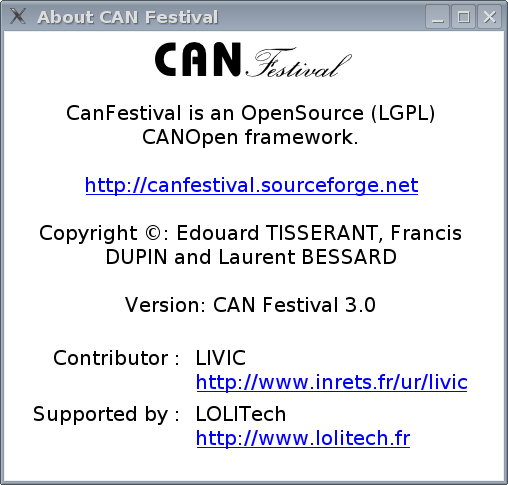
\includegraphics[width=7cm]{Pictures/10000201000001FC000001E5D65E8766} 
\par\end{center}


\subsubsection{Main view}

Top list let you choose dictionary section, bottom left list is the
selected index in that dictionary, and bottom right list are edited
sub -indexes.

\begin{center}
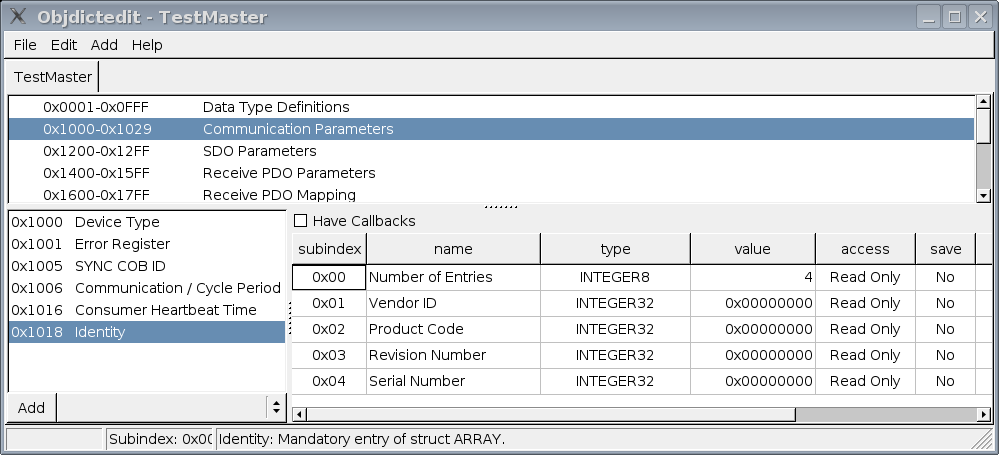
\includegraphics[width=12cm]{Pictures/10000201000003E7000001C7B0296577} 
\par\end{center}

\begin{center}
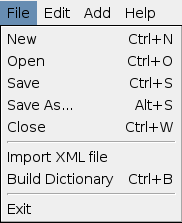
\includegraphics[width=3cm]{Pictures/10000000000000B6000000DF1EDD1E73} 
\par\end{center}

\begin{center}
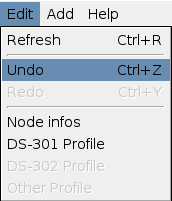
\includegraphics[width=3cm]{Pictures/10000000000000AC000000C9C3F53FA6} 
\par\end{center}

\begin{center}
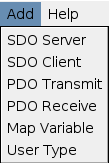
\includegraphics[width=3cm]{Pictures/100000000000006D000000A31EC8CB54} 
\par\end{center}

\begin{center}
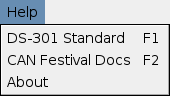
\includegraphics[width=3cm]{Pictures/10000000000000AA0000006014F74635} 
\par\end{center}


\subsubsection{New node}

Edit your node name and type. Choose your inherited specific profile.

\begin{center}
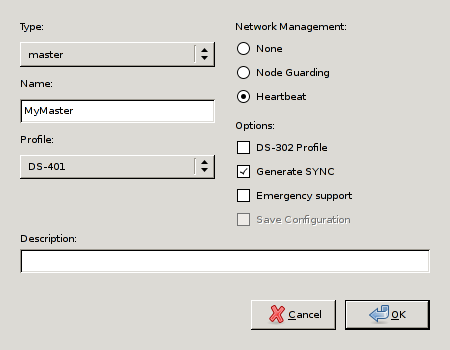
\includegraphics[width=11cm]{Pictures/new_node} 
\par\end{center}


\subsubsection{Node info}

Edit your node name and type.

\begin{center}
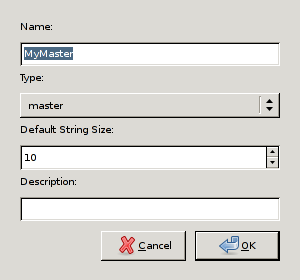
\includegraphics[width=7cm]{Pictures/node_info} 
\par\end{center}


\subsubsection{Profile editor}

Chose the used profile to edit.

\begin{center}
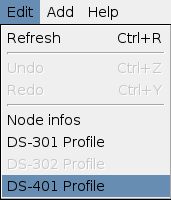
\includegraphics[width=4cm]{Pictures/10000000000000AB000000C88F594413} 
\par\end{center}

Pick up optional chosen profile entries.

\begin{center}
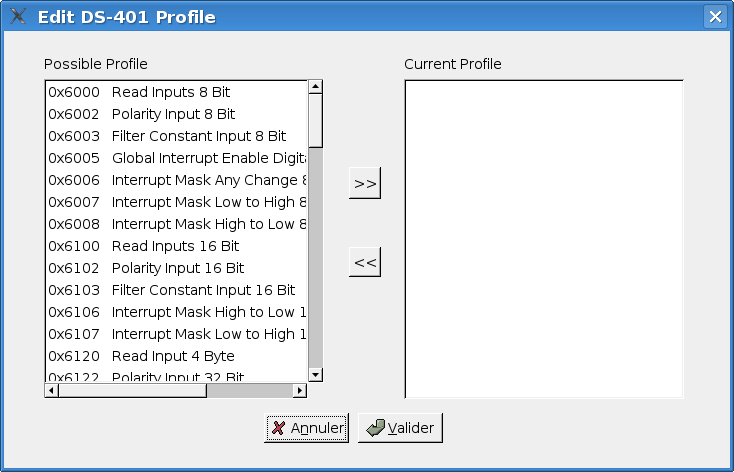
\includegraphics[width=11cm]{Pictures/10000201000002DE000001D82D89C224} 
\par\end{center}


\subsubsection{User types}

Use User Types to implement value boundaries, and string length

\begin{center}
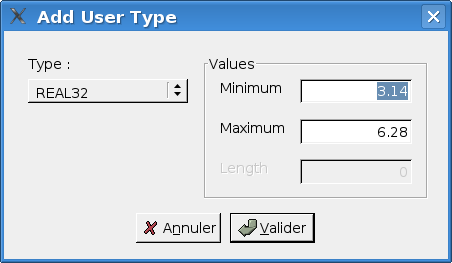
\includegraphics[width=11cm]{Pictures/10000201000001C40000010766961D7F} 
\par\end{center}


\subsubsection{Mapped variable}

Add your own specific dictionary entries and associated mapped variables.

\begin{center}
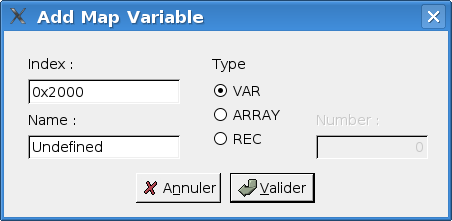
\includegraphics[width=11cm]{Pictures/10000201000001C4000000DD129D4661} 
\par\end{center}


\subsubsection{Integrated help}

Using F1 key, you can get context sensitive help.

\begin{center}
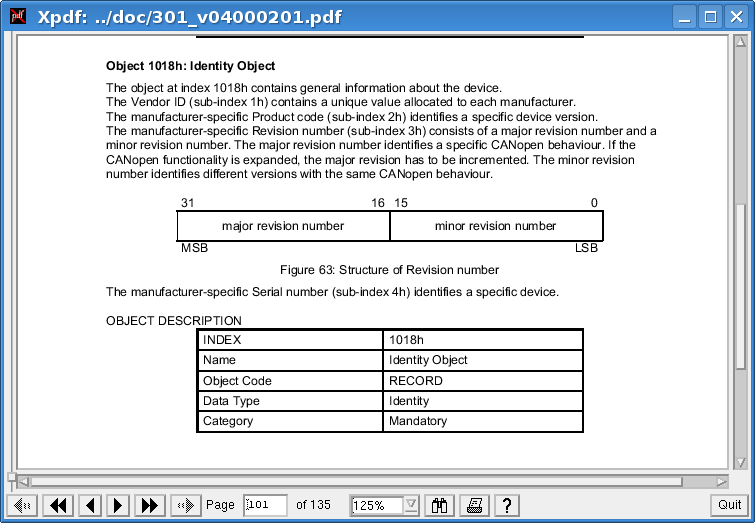
\includegraphics[width=12cm]{Pictures/10000201000002F30000020B23ED7F67} 
\par\end{center}

In order to do that, official 301\_v04000201.pdf file must be placed
into doc/ directory, and xpdf must be present on your system.

F2 key open HTML CanFestival help.

\begin{center}
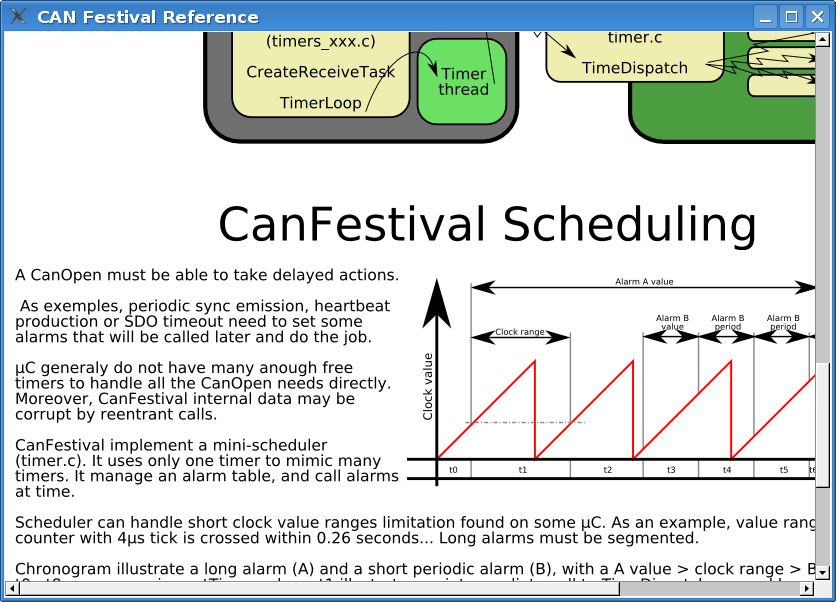
\includegraphics[width=12cm]{Pictures/10000201000003440000025ACC3FD2F1} 
\par\end{center}


\subsection{Generating the object Dictionary}

Once object dictionary has been edited and saved, you have to generate
object dictionary C code for your CanFestival node.


\subsubsection{With GUI}

Menu entry {}``File/Build Dictionary''.

\begin{center}
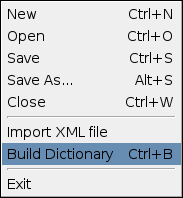
\includegraphics[width=4cm]{Pictures/10000201000000B7000000C66AF89CD5} 
\par\end{center}

Choose C file to create or overwrite. Header file will be also created
with the same prefix as C file.


\subsubsection{With command line}

\begin{verbatim}
	Usage of objdictgen.py :
	python objdictgen.py XMLFilePath CfilePath
\end{verbatim}



\section{FAQ}


\subsection{General}


\subsubsection{Does the code compiles on Windows ?}

Yes, with both Cygwin and Visual Studio C++. 

Because \canopen layer is coded with C, put a compilation option
/TC or /TP if you plan to mix C++ files. See the MSDN documentation
about that.


\subsubsection{How to fit the library to an other microcontr�ler ?}

First, be sure that you have at least 40K bytes of program memory,
and about 2k of RAM.

You have to create target specific interface to HW resources. Take
model on bundled interfaces provided in drivers/ and create your own
interface. You also have to update Makefile.in files for target specific
cflags and options. Choose {--}target= configure switch to compile
your specific interface.

You are welcome to contribute -back your own interfaces! Other Canfestival
users will use it and provide feedback, tests and enhancements.


\subsubsection{Is CanFestival3 conform to DS301 v.4.02 ?}

Thanks to Philippe Foureys (IUT of Valence), a slave node have been
tested with the National Instrument \canopen Conformance Test. It
passed the test with success.

Some very small unconformity have been found in very unusual situations,
for example in the SDO code response to wrong messages.


\subsection{LINUX}


\subsubsection{How to use a Peaksystem CAN board ?}

Just install peak driver and then compile and install Canfestival.
Peak driver is detected at compile time.


\subsubsection{How to use an unsupported CAN board ?}

You have to install the specific driver on your system, with necessary
libs and headers.

Use can\_peak.c/h or can\_virtual.c/h as an example, and adapt it
to your driver API.

Execute configure script and choose --can=mydriver


\subsection{Win32}

Compatibility:

\begin{enumerate}
\item Code was compiled MS VisualStudio 2003.NET and VisualStudio 2005.NET
for WindowsXP \ with ANSI and UNICODE configurations and for WindowsCE
5.0. 
\item Some preliminary testing was done, but not enough to be used in mission
critical projects. 
\end{enumerate}
Additional Features:

\begin{enumerate}
\item Non -integral integers support implementation UNS24, UNS40, UNS48
etc. 
\item When enable debug output with DEBUG\_WAR\_CONSOLE\_ON or DEBUG\_ERR\_CONSOLE\_ON,
you can navigate in CanFestival source code by double clicking at
diagnostic lines in VisualStudio.NET 200X Debug Output Window. 
\end{enumerate}
Custom size integral types such as INTEGER24, UNS40, INTEGER56 etc.
have been defined as 64 bits integers. You will need to replace sizeof(TYPE)
operators to sizeof\_TYPE definitions in generated code, i.e. replace
sizeof(UNS40) with sizeof\_UNS40.


\subsection{HCS12}


\subsubsection{Which board are you using ?}

A T -board from elektronikladen with a MC9S12DP256 or MC9S12DG256.


\subsubsection{Does the code compile with an other compiler than GNU gcc ?}

It is known to work with Metrowerks CodeWarrior. Here are some tips
from Philippe Foureys. :


\paragraph{Interrupt functions}


\subparagraph{Code for GCC:
}


\begin{verbatim}
	// prototype
	void __attribute__((interrupt))timer3Hdl(void):
	// function
	void __attribute__((interrupt))timer3Hdl(void){...}
\end{verbatim}

	
\subparagraph{Code for CodeWarrior
}


\begin{verbatim}
	// protoype
	void interrupt timer3Hdl(void);
	// function
	pragma CODE_SEG__NEAR_SEG_NON_BANKED
	void interrupt timer3Hdl(void)
	{...}
	pragma CODE_SEG_DEFAULT\end{verbatim}


\paragraph{Interrupt lock, unlock
}


\subparagraph{Code for GCC
}


\begin{verbatim}
 void unlock (void)
 {
   __asm__ __volatile__("cli");
 }
 void lock (void)
 {
   unsigned short mask;
   __asm__ __volatile__("tpa\n\tsei":"=d"(mask));
 }
\end{verbatim}


\subparagraph{Code for CodeWarrior}


\begin{verbatim}
void unlock (void)
	{
	  __asm("cli");
	}
	void lock (void)
	{
	  unsigned short mask;
	  __asm
	 {
	  tpa:tsei:"=d"(mask);
	 }
	}
\end{verbatim}


\paragraph{Initialize function}


\subparagraph{Code for GCC}


\begin{verbatim}
void initCanHCS12 (void)
{  
  //Init the HCS12 microcontroler for CanOpen 
  initHCS12();
   // Init the HCS12  CAN driver
  const canBusInit bi0 = {
    0,    /* no low power                 */ 
    0,    /* no time stamp                */
    1,    /* enable MSCAN                 */
    0,    /* clock source : oscillator (In fact, it is not used)   */
    0,    /* no loop back                 */
    0,    /* no listen only               */
    0,    /* no low pass filter for wk up */
  CAN_Baudrates[CAN_BAUDRATE_250K],
    {
      0x00,    /* Filter on 16 bits.
                  See Motorola Block Guide V02.14 fig 4-3 */
      0x00, 0xFF, /* filter 0 hight accept all msg      */
      0x00, 0xFF, /* filter 0 low accept all msg        */
      0x00, 0xFF, /* filter 1 hight filter all of  msg  */
      0x00, 0xFF, /* filter 1 low filter all of  msg    */
      0x00, 0xFF, /* filter 2 hight filter most of  msg */
      0x00, 0xFF, /* filter 2 low filter most of  msg   */
      0x00, 0xFF, /* filter 3 hight filter most of  msg */
      0x00, 0xFF, /* filter 3 low filter most of  msg   */
    }
};
\end{verbatim}


\subparagraph{Code for CodeWarrior
}


\begin{verbatim}
void initCanHCS12 (void)
{  
  //Init the HCS12 microcontroler for CanOpen 
  initHCS12();
   // Init the HCS12  CAN driver
  const canBusInit bi0 = {
    0,    /* no low power                 */ 
    0,    /* no time stamp                */
    1,    /* enable MSCAN                 */
    0,    /* clock source : oscillator (In fact, it is not used)   */
    0,    /* no loop back                 */
    0,    /* no listen only               */
    0,    /* no low pass filter for wk up */
    {
     1, /* clksrc */
     3, /* brp    */
     0, /* sjw    */
     0, /* samp   */
     1, /* tseg2  */
     12,/* tseg1  */
    },
    {
      0x00,    /* Filter on 16 bits.
                 See Motorola Block Guide V02.14 fig 4-3 */
      0x00, 0xFF, /* filter 0 hight accept all msg      */
      0x00, 0xFF, /* filter 0 low accept all msg        */
      0x00, 0xFF, /* filter 1 hight filter all of  msg  */
      0x00, 0xFF, /* filter 1 low filter all of  msg    */
      0x00, 0xFF, /* filter 2 hight filter most of  msg */
      0x00, 0xFF, /* filter 2 low filter most of  msg   */
      0x00, 0xFF, /* filter 3 hight filter most of  msg */
      0x00, 0xFF, /* filter 3 low filter most of  msg   */
    }
};
\end{verbatim}


\subsubsection{Does the code works in banked memory ?}

No. Today it seems that the port of gcc is bogged for using the banked
memory. So, unfortunately, we are limited to 48 Kbytes of memory code.


\subsubsection{What GCC version are you using ?}

We are using the stable RPM release 2.2 :

\begin{enumerate}
\item GNU Gcc 3.0.4. Build 20030501 
\item Newlib 1.10.0 Build 20030421 
\item GNU Binutils 2.12.1 Build 20030427 
\end{enumerate}

\section{Documentation resources}


\subsection{CIA : Can in Automation }

\href{http://www.can-cia.de/}{http://www.can -cia.de}


\subsection{Resources and training in \canopen 
}

\href{http://www.esacademy.com/}{http://www.esacademy.com}


\subsection{Elektronikladen HCS12 T -board }

\href{http://www.elektronikladen.de/en_hcs12tb.html}{http://www.elektronikladen.de/en\_hcs12tb.html}


\subsection{Gnu gcc compiler for HC12 }

\href{http://m68hc11.serveftp.org/m68hc11_port.php}{http://m68hc11.serveftp.org/m68hc11\_port.php}


\subsection{Motorola documentation on HC12 }

\href{http://www.freescale.com/webapp/sps/site/prod_summary.jsp?code=MC9S12DP256}{http://www.freescale.com/webapp/sps/site/prod\_summary.jsp?code=MC9S12DP256}


\subsection{Lauterbach debugger for HC12 }

\href{http://www.lauterbach.com/}{http://www.lauterbach.com}


\subsection{Python language }

\href{http://www.python.org/}{http://www.python.org}

\clearpage{}


\section{About the project}


\subsection{Contributors }

\begin{center}

\includegraphics[width=10cm]{Pictures/1000020100000258000000832C6FFAB4} 
\par\end{center}

Unit� mixte de recherche INRETS -LCPC

sur les Interractions V�hicule -Infrastructure -Conducteur

14, route de la mini�re

78000 Versailles

FRANCE

Tel : +33 1 40 43 29 01

\href{http://www.inrets.fr/ur/livic}{http://www.inrets.fr/ur/livic}

\textbf{Contributors :} Francis DUPIN

Camille BOSSARD

Laurent ROMIEUX

\bigskip{}

\textbf{Contributors :} Edouard TISSERANT (Original author)

Laurent BESSARD

\bigskip{}


Many thanks to the other contributors for their great work:

Raphael ZULLIGER

David DUMINY (st� A6R)

Zakaria BELAMRI


\subsection{Getting support}

Send your feedback and bug reports to \href{mailto:canfestival-devel@lists.sourceforge.net}{canfestival-devel@lists.sourceforge.net}.

\subsection{Contributing}

You are free to contribute your specific interfaces back to the project.
This way, you can hope to get support from CanFestival users community.

Please send your patch to \href{mailto:canfestival-devel@lists.sourceforge.net}{canfestival
-devel@lists.sourceforge.net}.

Feel free to create some new predefined DS -4xx profiles ({*}.prf)
in objdictgen/config, as much as possible respectful to the official
specifications.


\subsection{License}

All the project is licensed with LGPL. This mean you can link CanFestival
with any code without being obliged to publish it.


\begin{verbatim}
#This file is part of CanFestival, a library implementing CanOpen Stack. 
# 
#Copyright (C): Edouard TISSERANT, Francis DUPIN and Laurent BESSARD 
# 
#See COPYING file for copyrights details. 
# 
#This library is free software; you can redistribute it and/or 
#modify it under the terms of the GNU Lesser General Public 
#License as published by the Free Software Foundation; either 
#version 2.1 of the License, or (at your option) any later version. 
# 
#This library is distributed in the hope that it will be useful, 
#but WITHOUT ANY WARRANTY; without even the implied warranty of 
#MERCHANTABILITY or FITNESS FOR A PARTICULAR PURPOSE.  See the GNU 
#Lesser General Public License for more details. 
# 
#You should have received a copy of the GNU Lesser General Public 
#License along with this library; if not, write to the Free Software 
#Foundation, Inc., 59 Temple Place, Suite 330, Boston, MA  02111-1307  USA 
\end{verbatim}


\end{document}
